\newpage
\title{}
\author{}
\hspace{0.075em}
\begin{tikzpicture}
  %\initializesizeandshifts
  %\setxshift{-60}
   %\setyshift{2}

  %% the title block, #1 - shift, the default value is (0,0), #2 - width, #3 - scale
  %% the alias of the title block is `title', so we can refer to its boundaries later
  %\ifthenelse{\equal{\template}{1}}{ 
  %  \titleblock{60}{0}
  %}{
  %  \titleblock{60}{0}
  %}


  %frame/.style={rounded corners=30, line width=0.4cm, inner sep=1cm},
  %frametwo/.style={thick, inner sep=1cm, %
  %  drop shadow={shadow xshift=0.2cm, shadow yshift=-0.2cm, opacity=0.3}, %
  %  decorate, decoration={random steps,segment length=1cm,amplitude=0.15cm}
    % decorate, decoration={penciline,amplitude=0.2cm}
  %},% 

  %%%%%%%%%% ------------------------------------------ %%%%%%%%%%
\blocknodew[($(currenty)-(-0.5,0)$)]{84.5}{已开展的研究工作(一)} %
 {   
\begin{minipage}{0.54\linewidth}
\coloredbox{colorone!50!}{
\begin{center}
\begin{minipage}[t]{0.49\linewidth}
\coloredbox{colorthree!50!}{
\begin{tikzfigure}[球形液滴的形成]
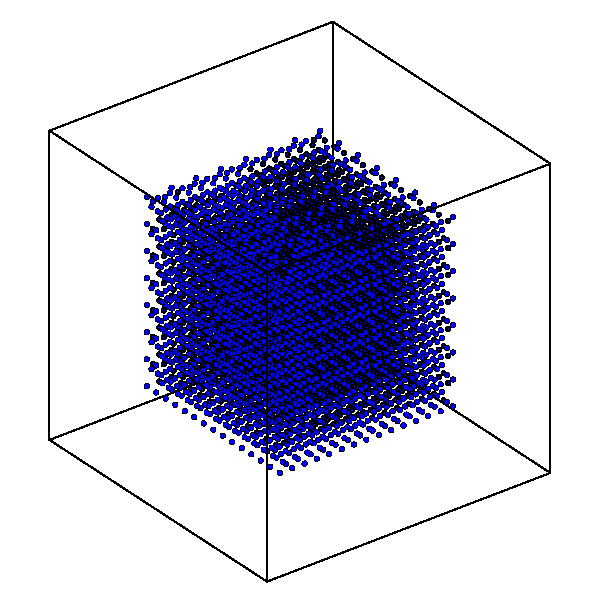
\includegraphics[width=0.3875\textwidth]{./figures/drop/1.pdf}
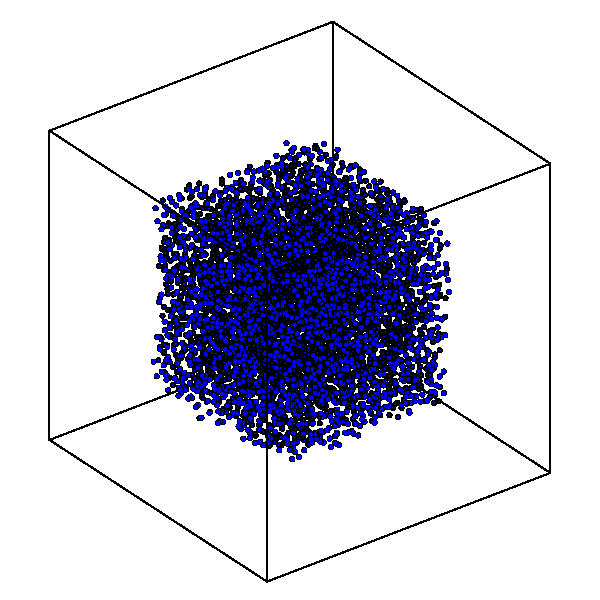
\includegraphics[width=0.3875\textwidth]{./figures/drop/4.pdf}\\
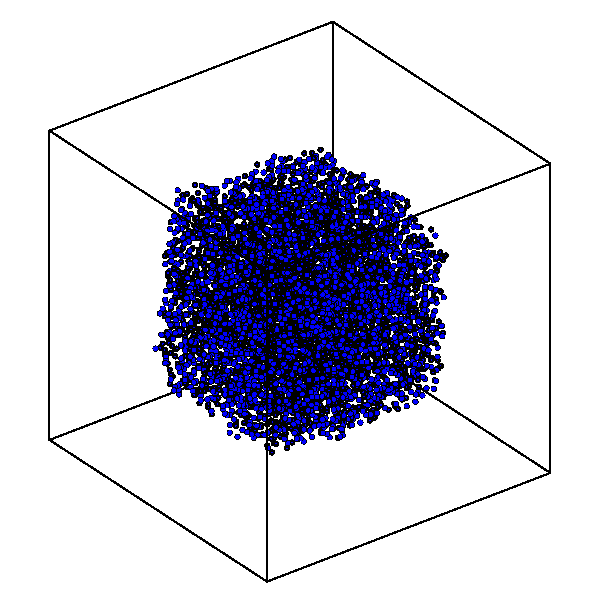
\includegraphics[width=0.3875\textwidth]{./figures/drop/7.pdf}
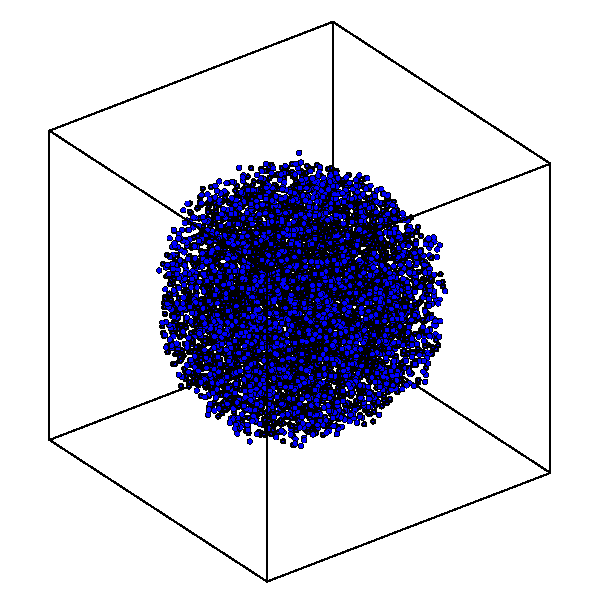
\includegraphics[width=0.3875\textwidth]{./figures/drop/10.pdf}
\end{tikzfigure}}
\end{minipage}
\begin{minipage}[t]{0.49\linewidth}
\coloredbox{colorthree!50!}{
\begin{tikzfigure}[液滴接触角的模拟]
\usetikzlibrary{%
    decorations.pathreplacing,%
    decorations.pathmorphing,arrows
}
\begin{tikzpicture}[rounded corners=0em,decoration={random steps,segment length=10em,amplitude=0},scale=1.65,line width= 0.1em, clip=true]
%\draw(-1.5,-1.2) rectangle (10,8.25);
\clip(-1.5,-1.2) rectangle (10,8.25);
  \begin{axis}[xmin=-40, xmax=-15, ymin=0, ymax=180, width=320pt, height=275pt,
              ytick={0,30,60,90,120,150,180},
              xlabel={$A_{sl}$}, ylabel={$\theta$},
              tick label style={font=\tiny},
              label style={font=\tiny},
              ylabel style={yshift=20pt},
              xlabel style={yshift=10pt},
              xticklabel style={yshift=12pt},
              yticklabel style={xshift=10pt},clip=true
              ]
   \addplot[only marks, mark=*, draw=black, fill=black!30, mark size=1.5]  coordinates {
           (-40,0) (-37.5,30) (-35, 55) (-32.5,75) (-30,90) 
           (-27.5, 100) (-25,111) (-22.5,122) (-20,133) (-17.5, 150)};
  \addplot[thick,black] coordinates {
           (-40,0) (-37.5,30) (-35, 55) (-32.5,75) (-30,90) 
           (-27.5, 100) (-25,111) (-22.5,122) (-20,133) (-17.5, 150)};

  \end{axis}
\begin{scope}[ media/.style={font={\tiny\sffamily}},
    wave/.style={
        decorate,decoration={snake,post length=1.4mm,amplitude=2mm,
        segment length=2mm},thick},
    interface/.style={
        postaction={draw,decorate,decoration={border,angle=-45,
                    amplitude=0.3cm,segment length=2mm}}},xshift=70,yshift=130,scale=1.25]

\draw[fill=blue!20,semithick](20:1) arc(20:160:1);
\draw[semithick,interface] (-1.5,0.35)--(1.5,0.35);

\draw[semithick,blue](160:1)--++(70:0.75);
\draw[blue] (160:1)++(0.2,0)  arc(0:70:0.2) node[right]{\tiny $\theta$};

\node[above=-5] at (-0.4,-3.7) {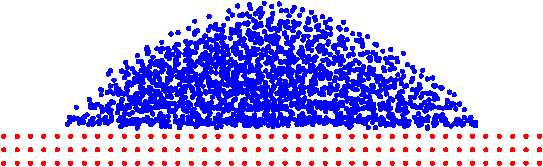
\includegraphics[width=5em]{./figures/35.pdf}};
\node[above=-5] at (4.2,-3.7) {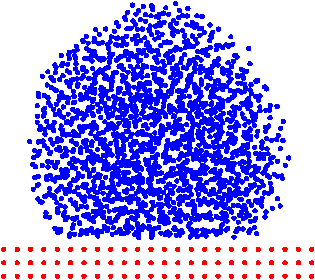
\includegraphics[width=3em]{./figures/20.pdf}};
\end{scope}
\end{tikzpicture}

\end{tikzfigure}}
\end{minipage}
\end{center}
\vspace{-30pt}
\begin{center}
\begin{minipage}[t]{0.49\linewidth}
\coloredbox{colorthree!50!}{
\begin{tikzfigure}[纤维阵列中细胞的模拟示意图]
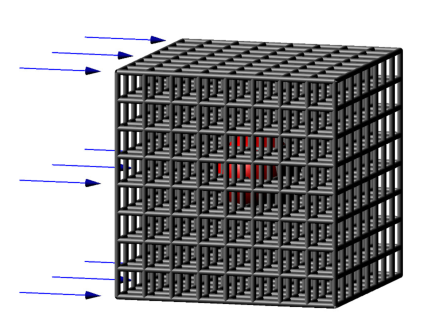
\includegraphics[width=0.975\textwidth]{./figures/matrix.pdf}
\end{tikzfigure}}
\end{minipage}
\begin{minipage}[t]{0.49\linewidth}
\coloredbox{colorthree!50!}{
\begin{tikzfigure}[刚体圆球绕流的阻力系数]
\begin{tikzpicture}[rounded corners=0em,decoration={random steps,segment length=10em,amplitude=0},scale=1.65,line width= 0.1em, clip=true]
\clip(-1.5,-1.2) rectangle (10,8.25);
%\draw(-1.5,-1.2) rectangle (10,8);
\begin{loglogaxis}[xmin=0.1, xmax=1000, ymin=0.01, ymax=10000, width=320pt, height=275pt,
xlabel=$\mathrm{Re}$,ylabel=$C_d$,
legend style={cells={anchor=west},font=\tiny},
              tick label style={font=\tiny},
              label style={font=\tiny},
              ylabel style={yshift=20pt},
              xlabel style={yshift=10pt},
              xticklabel style={yshift=12pt},
              yticklabel style={xshift=10pt},clip=true
]

\addplot[only marks, draw=black, fill=black!30, mark size=2] coordinates {
		( 0.20,112.34)
                ( 0.99, 27.33)
                ( 2.10, 13.01)
                ( 4.02,  7.04)
                ( 9.80,  3.28)
                ( 22.00, 2.02)
                ( 40.98, 1.31)
                ( 81.32, 0.98)
                (101.25, 0.99)};
\addlegendentry{DPD}

\addplot+[mark=none,domain=0.1:1000,samples=2,densely dashed,red] {24/x}; 
\addlegendentry{$24/\mathrm{Re}$}
%\addlegendentry{$\frac{24}{\mathrm{Re}}$}


\addplot+[mark=none,domain=0.2:1000,samples=200,smooth,blue] {21.12/x + 6.3/sqrt(x) + 0.25}; 
\addlegendentry{$21.12/\mathrm{Re}+6.3/\sqrt{\mathrm{Re}}+0.25$}
%\addlegendentry{$\frac{21.12}{\mathrm{Re}}+\frac{6.3}{\sqrt{\mathrm{Re}}}+0.25$}

\end{loglogaxis}
\end{tikzpicture}

\end{tikzfigure}}
\end{minipage}
\end{center}
\vspace{-35pt}
}
\end{minipage}
\begin{minipage}{0.005\linewidth}
  {~}
\end{minipage}
\begin{minipage}{0.45\linewidth}
\coloredbox{colorone!50!}{
\begin{itemize}
\item 图4. 在表面张力的作用下, 液滴由立方体转变为球形. 传统的DPD仅能模拟多体系统中液-液及液-固界面特性. 通过引入新型作用势和多体DPD模型, 实现多相流动系统中微重力, 粘性力, 表面张力及毛细力相互作用的模拟.
\item 图5. 调整多体DPD中液体粒子和固壁粒子间的作用力参数可实现不同接触角的模拟. 通过引入新型作用势或多体DPD, 可实现不同性质流体的模拟. 
\item 图6. 通过加入刚体模型, 模拟不同孔隙率的圆柱阵列对流体流动的影响, 并以此来初步研究细胞外纤维基质对细胞受体液流体作用力的屏蔽作用. 
\item 图7. 应用刚体模型研究球体绕流, 将结果与理论解和实验结果对比. 此外还研究了圆柱绕流和含运动颗粒的流动. 
\end{itemize}
}
\vspace{-0.5em}

\coloredbox{colorone!50!}{
{\Large\bfseries\textcolor{blocktitletextcolor}{小结}}\vspace{0.25em}
\small

\begin{itemize}
\item 应用新型保守势和改进的DPD模型, 实现了不同性质流体的模拟.
\item 通过引入刚体模型, 初步研究了细胞外纤维基质对细胞受间质流体作用力的屏蔽作用.
\end{itemize}

\vspace{0.75em}
{\Large\bfseries\textcolor{blocktitletextcolor}{发表的相关文章}}\vspace{0.5em}
\small

\begin{basedescript}{\desclabelstyle{\pushlabel}\desclabelwidth{1em}}
\item[1.] Zhou L. V., Liu M. B. and Chang, J. Z., Acta Polymerica Sinica 7: 720-727, 2012.
\item[2.] Liu M.B., Liu G.R., Zhou L. V. and Chang J. Z., Archives of Computational Methods in Engineering.(2014. Accept)
\end{basedescript}
}
\end{minipage}
}


%%%%%%%%%% ------------------------------------------ %%%%%%%%%%
\blocknodew[($(currenty)-(0,0)$)]{84.5}{已开展的研究工作(二)} 
{   
\begin{minipage}{0.54\linewidth}
\coloredbox{colorone!50!}{
\begin{center}
\begin{minipage}[t]{0.49\linewidth}
\coloredbox{colorthree!50!}{
\begin{tikzfigure}[微缩通道中高分子链的模拟]
%\includegraphics[width=0.975\textwidth]{./figures/chainY4000s.pdf}
\usetikzlibrary{%
    decorations.pathreplacing,%
    decorations.pathmorphing,arrows
}
\begin{tikzpicture}[rounded corners=0em,decoration={random steps,segment length=10em,amplitude=0},scale=1.65,line width= 0.1em, clip=true]
%\draw(-1.5,-1.2) rectangle (10,8);
\clip(-1.5,-1.2) rectangle (10,8.25);
  \begin{axis}[xmin=-30, xmax=30, ymin=-25, ymax=25, width=320pt, height=275pt,
              ytick={-15,-5,0,5,15},
              xlabel={$x$}, ylabel={$z$},
              tick label style={font=\tiny},
              label style={font=\tiny},
              ylabel style={yshift=10pt},
              xlabel style={yshift=10pt},
              xticklabel style={yshift=12pt},
              yticklabel style={xshift=10pt},clip=true
              ]

   \addplot[color=blue,no marks, dashed, thick] coordinates {(25.5,-25) (25.5,25)};
   \addplot[color=red,no marks, dashed, thick] coordinates {(16.5,-25) (16.5,25)};
   \addplot[color=black,no marks, dashed, thick] coordinates {(0,-25) (0,25)};
   \addplot[color=purple,no marks, dashed, thick] coordinates {(-16.5,-25) (-16.5,25)};
   \addplot[color=brown!50!black,no marks, dashed, thick] coordinates {(-25.5,-25) (-25.5,25)};





   \addplot[only marks, mark=ball, ball color=gray,mark size=1.25]  table[x=wx,y=wz]{./figures/data/wallpartice.dat};

   \addplot[no marks, red, line width=0.015em]  table[x=x1,y=y1]{./figures/data/DNA30new.dat};
   \addplot[only marks, mark=ball, ball color=red, mark size=1.25]  table[x=x1,y=y1]{./figures/data/DNA30new.dat};

   \addplot[no marks, red, line width=0.015em]  table[x=x2,y=y2]{./figures/data/DNA30new.dat};
   \addplot[only marks, mark=ball, ball color=red, mark size=1.25]  table[x=x2,y=y2]{./figures/data/DNA30new.dat};

   \addplot[no marks, red, line width=0.015em]  table[x=x3,y=y3]{./figures/data/DNA30new.dat};
   \addplot[only marks, mark=ball, ball color=red, mark size=1.25]  table[x=x3,y=y3]{./figures/data/DNA30new.dat};

   \addplot[no marks, red, line width=0.015em]  table[x=x4,y=y4]{./figures/data/DNA30new.dat};
   \addplot[only marks, mark=ball, ball color=red, mark size=1.25]  table[x=x4,y=y4]{./figures/data/DNA30new.dat};

   \addplot[no marks, red, line width=0.015em]  table[x=x5,y=y5]{./figures/data/DNA30new.dat};
   \addplot[only marks, mark=ball, ball color=red, mark size=1.25]  table[x=x5,y=y5]{./figures/data/DNA30new.dat};




   \addplot[no marks, blue, line width=0.015em]  table[x=x6,y=y6]{./figures/data/DNA30new.dat};
   \addplot[only marks, mark=ball, ball color=blue, mark size=1.25]  table[x=x6,y=y6]{./figures/data/DNA30new.dat};

   \addplot[no marks, blue, line width=0.015em]  table[x=x7,y=y7]{./figures/data/DNA30new.dat};
   \addplot[only marks, mark=ball, ball color=blue, mark size=1.25]  table[x=x7,y=y7]{./figures/data/DNA30new.dat};

   \addplot[no marks, blue, line width=0.015em]  table[x=x8,y=y8]{./figures/data/DNA30new.dat};
   \addplot[only marks, mark=ball, ball color=blue, mark size=1.25]  table[x=x8,y=y8]{./figures/data/DNA30new.dat};

   \addplot[no marks, blue, line width=0.015em]  table[x=x9,y=y9]{./figures/data/DNA30new.dat};
   \addplot[only marks, mark=ball, ball color=blue, mark size=1.25]  table[x=x9,y=y9]{./figures/data/DNA30new.dat};

   \addplot[no marks, blue, line width=0.015em]  table[x=x10,y=y10]{./figures/data/DNA30new.dat};
   \addplot[only marks, mark=ball, ball color=blue, mark size=1.25]  table[x=x10,y=y10]{./figures/data/DNA30new.dat};



   \addplot[no marks, green, line width=0.015em]  table[x=x11,y=y11]{./figures/data/DNA30new.dat};
   \addplot[only marks, mark=ball, ball color=green, mark size=1.25]  table[x=x11,y=y11]{./figures/data/DNA30new.dat};

   \addplot[no marks, green, line width=0.015em]  table[x=x12,y=y12]{./figures/data/DNA30new.dat};
   \addplot[only marks, mark=ball, ball color=green, mark size=1.25]  table[x=x12,y=y12]{./figures/data/DNA30new.dat};

   \addplot[no marks, green, line width=0.015em]  table[x=x13,y=y13]{./figures/data/DNA30new.dat};
   \addplot[only marks, mark=ball, ball color=green, mark size=1.25]  table[x=x13,y=y13]{./figures/data/DNA30new.dat};

   \addplot[no marks, green, line width=0.015em]  table[x=x14,y=y14]{./figures/data/DNA30new.dat};
   \addplot[only marks, mark=ball, ball color=green, mark size=1.25]  table[x=x14,y=y14]{./figures/data/DNA30new.dat};

   \addplot[no marks, green, line width=0.015em]  table[x=x15,y=y15]{./figures/data/DNA30new.dat};
   \addplot[only marks, mark=ball, ball color=green, mark size=1.25]  table[x=x15,y=y15]{./figures/data/DNA30new.dat};




   \addplot[no marks, brown, line width=0.015em]  table[x=x16,y=y16]{./figures/data/DNA30new.dat};
   \addplot[only marks, mark=ball, ball color=brown, mark size=1.25]  table[x=x16,y=y16]{./figures/data/DNA30new.dat};

   \addplot[no marks, brown, line width=0.015em]  table[x=x17,y=y17]{./figures/data/DNA30new.dat};
   \addplot[only marks, mark=ball, ball color=brown, mark size=1.25]  table[x=x17,y=y17]{./figures/data/DNA30new.dat};

   \addplot[no marks, brown, line width=0.015em]  table[x=x18,y=y18]{./figures/data/DNA30new.dat};
   \addplot[only marks, mark=ball, ball color=brown, mark size=1.25]  table[x=x18,y=y18]{./figures/data/DNA30new.dat};

   \addplot[no marks, brown, line width=0.015em]  table[x=x19,y=y19]{./figures/data/DNA30new.dat};
   \addplot[only marks, mark=ball, ball color=brown, mark size=1.25]  table[x=x19,y=y19]{./figures/data/DNA30new.dat};

   \addplot[no marks, brown, line width=0.015em]  table[x=x20,y=y20]{./figures/data/DNA30new.dat};
   \addplot[only marks, mark=ball, ball color=brown, mark size=1.25]  table[x=x20,y=y20]{./figures/data/DNA30new.dat};

   \addplot[no marks, purple, line width=0.015em]  table[x=x21,y=y21]{./figures/data/DNA30new.dat};
   \addplot[only marks, mark=ball, ball color=purple, mark size=1.25]  table[x=x21,y=y21]{./figures/data/DNA30new.dat};

   \addplot[no marks, purple, line width=0.015em]  table[x=x22,y=y22]{./figures/data/DNA30new.dat};
   \addplot[only marks, mark=ball, ball color=purple, mark size=1.25]  table[x=x22,y=y22]{./figures/data/DNA30new.dat};

   \addplot[no marks, purple, line width=0.015em]  table[x=x23,y=y23]{./figures/data/DNA30new.dat};
   \addplot[only marks, mark=ball, ball color=purple, mark size=1.25]  table[x=x23,y=y23]{./figures/data/DNA30new.dat};

   \addplot[no marks, purple, line width=0.015em]  table[x=x24,y=y24]{./figures/data/DNA30new.dat};
   \addplot[only marks, mark=ball, ball color=purple, mark size=1.25]  table[x=x24,y=y24]{./figures/data/DNA30new.dat};

   \addplot[no marks, purple, line width=0.015em]  table[x=x25,y=y25]{./figures/data/DNA30new.dat};
   \addplot[only marks, mark=ball, ball color=purple, mark size=1.25]  table[x=x25,y=y25]{./figures/data/DNA30new.dat};




   \addplot[no marks, magenta, line width=0.015em]  table[x=x26,y=y26]{./figures/data/DNA30new.dat};
   \addplot[only marks, mark=ball, ball color=magenta, mark size=1.25]  table[x=x26,y=y26]{./figures/data/DNA30new.dat};

   \addplot[no marks, magenta, line width=0.015em]  table[x=x27,y=y27]{./figures/data/DNA30new.dat};
   \addplot[only marks, mark=ball, ball color=magenta, mark size=1.25]  table[x=x27,y=y27]{./figures/data/DNA30new.dat};

   \addplot[no marks, magenta, line width=0.015em]  table[x=x28,y=y28]{./figures/data/DNA30new.dat};
   \addplot[only marks, mark=ball, ball color=magenta, mark size=1.25]  table[x=x28,y=y28]{./figures/data/DNA30new.dat};

   \addplot[no marks, magenta, line width=0.015em]  table[x=x29,y=y29]{./figures/data/DNA30new.dat};
   \addplot[only marks, mark=ball, ball color=magenta, mark size=1.25]  table[x=x29,y=y29]{./figures/data/DNA30new.dat};

   \addplot[no marks, magenta, line width=0.015em]  table[x=x30,y=y30]{./figures/data/DNA30new.dat};
   \addplot[only marks, mark=ball, ball color=magenta, mark size=1.25]  table[x=x30,y=y30]{./figures/data/DNA30new.dat};

  \end{axis}
\end{tikzpicture}

%\includegraphics[width=0.97\textwidth]{./figures/Tprof.pdf}
\end{tikzfigure}}
\end{minipage}
\begin{minipage}[t]{0.49\linewidth}
\coloredbox{colorthree!50!}{
\begin{tikzfigure}[速度, 密度和温度曲线]
%\includegraphics[width=0.97\textwidth]{./figures/Tprof.pdf}
\usetikzlibrary{%
    decorations.pathreplacing,%
    decorations.pathmorphing,arrows
}
\begin{tikzpicture}[rounded corners=0.em,decoration={random steps,segment length=10em,amplitude=0},scale=1.65,line width= 0.1em, clip=true]
%\draw(-1.5,-1.2) rectangle (10,8.25);
\clip(-1.5,-1.2) rectangle (10,8.25);
\begin{scope}[yshift=130pt]
  \begin{axis}[xmin=-15, xmax=15, ymin=-0.1, ymax=1.2, width=320pt, height=140pt,
              ytick={0,0.2,0.4,0.6,0.8,1},
              %xlabel={$z$}, 
              ylabel={$v_x$},
              xticklabel=\empty,
              tick label style={font=\tiny},
              label style={font=\tiny},
              ylabel style={yshift=20pt},
              %xlabel style={yshift=10pt},
              %xticklabel style={yshift=12pt},
              yticklabel style={xshift=10pt},
              clip=true,thick,
             legend style={font=\tiny, cells={anchor=west}},
              ]
   \addplot[no marks, blue]  table[x=z,y=v]{./figures/data/DNAprofile1.dat};
   %\addlegendentry{$x = 25.5$};
   \addplot[no marks, red]  table[x=z,y=v]{./figures/data/DNAprofile2.dat};
   %\addlegendentry{$x = 16.5$};
   \addplot[no marks, black]  table[x=z,y=v]{./figures/data/DNAprofile3.dat};
   %\addlegendentry{$x = 0$};
   \addplot[no marks, purple]  table[x=z,y=v]{./figures/data/DNAprofile4.dat};
   %\addlegendentry{$x = -16.5$};
   \addplot[no marks, brown!50!black]  table[x=z,y=v]{./figures/data/DNAprofile5.dat};
   %\addlegendentry{$x = -25.5$};
   
   \addplot[color=gray,no marks, dashed] coordinates {(-5,-1) (-5,1.5)};
   \addplot[color=gray,no marks, dashed] coordinates {(5,-1) (5,1.5)};
  \end{axis}
\end{scope}

\begin{scope}[yshift=80pt]
\begin{axis}[xmin=-15, xmax=15, ymin=0.75, ymax=1.25, width=320pt, height=90pt,
              ytick={0.8,1,1.2},
              %xlabel={$z$}, 
              ylabel={$T$},
              xticklabel=\empty,
              tick label style={font=\tiny},
              label style={font=\tiny},
              ylabel style={yshift=20pt},
              %xlabel style={yshift=10pt},
              %xticklabel style={yshift=12pt},
              yticklabel style={xshift=10pt},
              clip=true,thick
              ]
   \addplot[no marks, blue]  table[x=z,y=t]{./figures/data/DNAprofile1.dat};
   \addplot[no marks, red]  table[x=z,y=t]{./figures/data/DNAprofile2.dat};
   \addplot[no marks, black]  table[x=z,y=t]{./figures/data/DNAprofile3.dat};
   \addplot[no marks, purple]  table[x=z,y=t]{./figures/data/DNAprofile4.dat};
   \addplot[no marks, brown!50!black]  table[x=z,y=t]{./figures/data/DNAprofile5.dat};
   \addplot[color=gray,no marks, dashed] coordinates {(-5,0) (-5,1.5)};
   \addplot[color=gray,no marks, dashed] coordinates {(5,0) (5,1.5)};
  \end{axis}
\end{scope}

\begin{scope}[yshift=0pt]
\begin{axis}[xmin=-15, xmax=15, ymin=1.5, ymax=4.75, width=320pt, height=120pt,
              ytick={2,3,4},
              xlabel={$z$}, 
              ylabel={$\rho$},
              tick label style={font=\tiny},
              label style={font=\tiny},
              ylabel style={yshift=20pt},
              xlabel style={yshift=10pt},
              xticklabel style={yshift=12pt},
              yticklabel style={xshift=10pt},
              clip=true,thick
              ]
   \addplot[no marks, blue]  table[x=z,y=rho]{./figures/data/DNAprofile1.dat};
   \addplot[no marks, red]  table[x=z,y=rho]{./figures/data/DNAprofile2.dat};
   \addplot[no marks, black]  table[x=z,y=rho]{./figures/data/DNAprofile3.dat};
   \addplot[no marks, purple]  table[x=z,y=rho]{./figures/data/DNAprofile4.dat};
   \addplot[color=gray,no marks, dashed] coordinates {(-5,1) (-5,5)};
   \addplot[color=gray,no marks, dashed] coordinates {(5,1) (5,5)};
  \end{axis}
\end{scope}

\end{tikzpicture}

\end{tikzfigure}}
\end{minipage}
\end{center}
\vspace{-45pt}
\begin{center}
\begin{minipage}[t]{0.49\linewidth}
\coloredbox{colorthree!50!}{
\begin{tikzfigure}[红细胞模型和模拟]
%\begin{tikzpicture}[scale=1,x=1em,y=1em]
\node at (0,0) {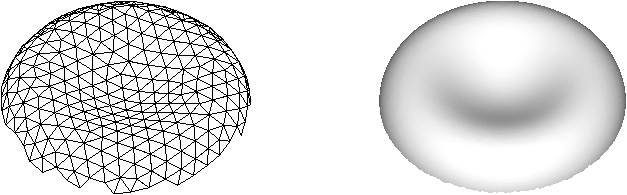
\includegraphics[width=11em]{./figures/network2continuum.pdf}};
\draw[very thick, <->, >=stealth'] (-2,0.5) node[text width=4.5em,left] {\tiny 弹簧常数, 弯曲常数\vspace{-1em} 体积约束, 面积约束} -- (2, 0.5) node[text width=4.5em, right] {\tiny 剪切模量, 压缩模量\vspace{-1em} 杨氏模量, 弯曲刚度};
%\draw[very thick, <->, >=stealth'] (-0.8,0) -- (0.8, 0);
\draw[very thick, <->, >=stealth'] (-2,-4.5) node[left]{\scriptsize 粒子模型} -- (2, -4.5) node[right] {\scriptsize 连续模型};;
\end{tikzpicture}

\innerblockplain[colorone!80!]{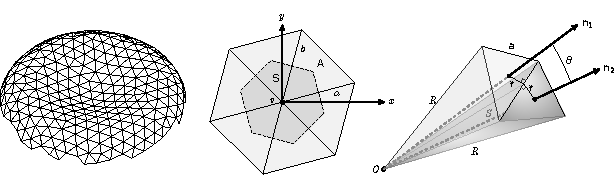
\includegraphics[width=\textwidth]{./figures/rbcmodel.pdf}}
\vspace{-0.15em}

\innerblockplain[colorone!80!]{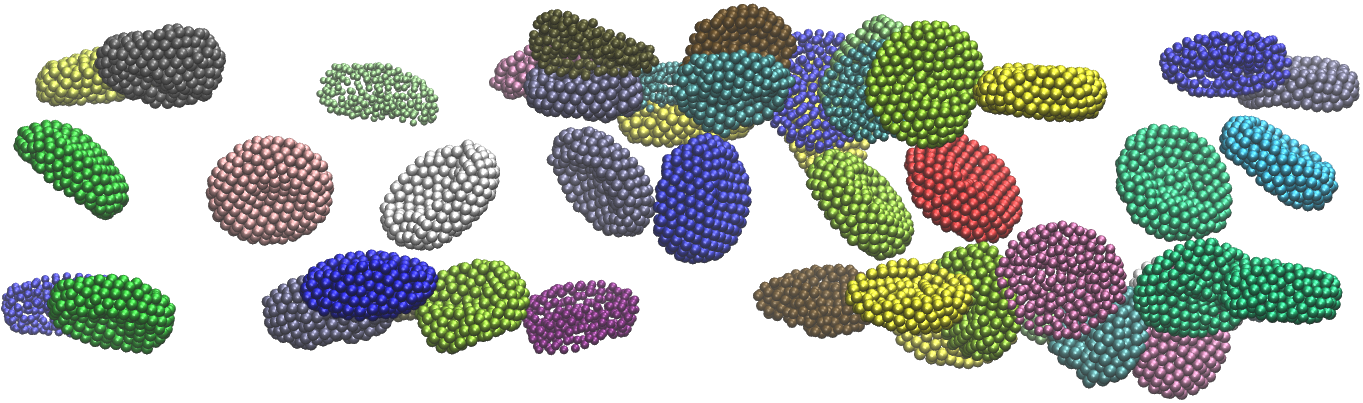
\includegraphics[width=\textwidth]{./figures/rbc.png}}
\vspace{-0.85em}
%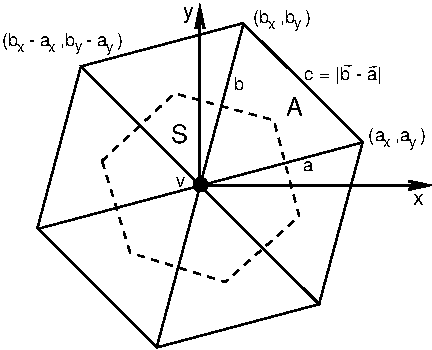
\includegraphics[width=0.4\textwidth]{./figures/hexagonalcell.pdf}
%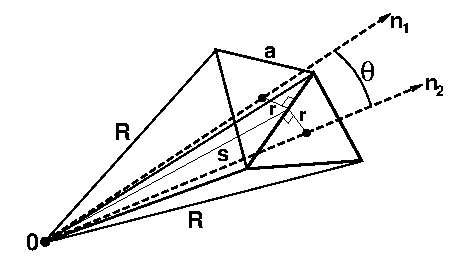
\includegraphics[width=0.55\textwidth]{./figures/bend.pdf}
\end{tikzfigure}}
\end{minipage}
\begin{minipage}[t]{0.49\linewidth}
\coloredbox{colorthree!50!}{
\begin{tikzfigure}[癌细胞通过微缩通道的构型]
%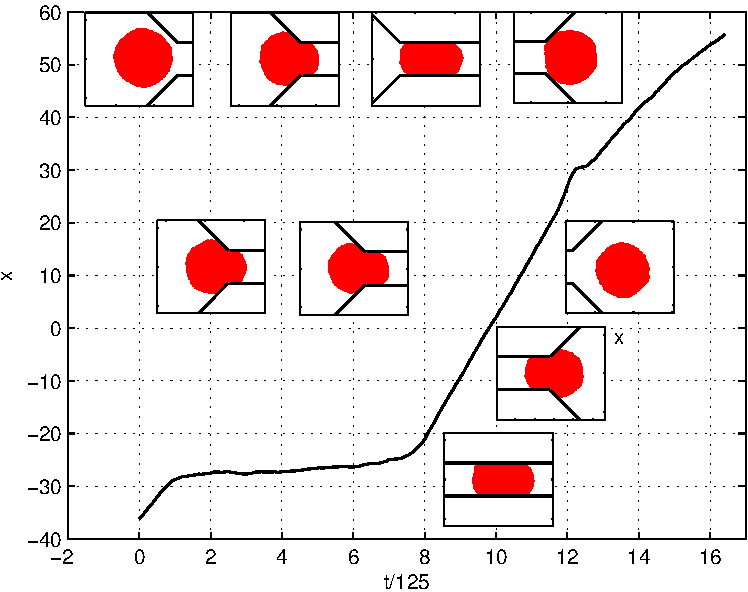
\includegraphics[width=\textwidth]{./figures/x.pdf}
\usetikzlibrary{%
    decorations.pathreplacing,%
    decorations.pathmorphing,arrows
}
\begin{tikzpicture}[rounded corners=0em,decoration={random steps,segment length=10em,amplitude=0},scale=1.65,line width= 0.1em, clip=true]
%\draw(-1.5,-1.2) rectangle (10,8.25);
\clip(-1.5,-1.2) rectangle (10,8.25);
\begin{scope}[yshift=130pt]
  \begin{axis}[xmin=-60, xmax=60, ymin=-20.75, ymax=20.75, width=320pt, height=140pt,
              ytick={-20,0,20},
              %xlabel={$t$}, 
              ylabel={$z$},
              xticklabel=\empty,
              tick label style={font=\tiny},
              label style={font=\tiny},
              ylabel style={yshift=20pt},
             % xlabel style={yshift=10pt},
              xticklabel style={yshift=12pt},
              yticklabel style={xshift=10pt},clip=true
              ]

   \addplot[color=black,no marks,thick] coordinates {(-70,-20.25) (-40,-22.25) (-23, -3.25) (23, -3.25) (40,-20.25) (70,-20.25)};
   \addplot[color=black,no marks,thick] coordinates {(-70,20.25) (-40,20.25) (-23, 3.25) (23, 3.25) (40,20.25) (70,20.25)};

   \addplot[no marks,ball color=red]  table[x=x1,y=y1]{./figures/data/cellshape.dat};
   \addplot[no marks, blue!25!red,thick]  table[x=x2,y=y2]{./figures/data/cellshape.dat};
   \addplot[no marks, blue!50!red,thick]  table[x=x3,y=y3]{./figures/data/cellshape.dat};
   \addplot[no marks, blue!75!red,thick]  table[x=x4,y=y4]{./figures/data/cellshape.dat};
   \addplot[no marks, blue!100!red,thick]  table[x=x5,y=y5]{./figures/data/cellshape.dat};
   \addplot[no marks, blue!75!green,thick]  table[x=x6,y=y6]{./figures/data/cellshape.dat};
   \addplot[no marks, blue!50!green,thick]  table[x=x7,y=y7]{./figures/data/cellshape.dat};
   \addplot[no marks, blue!25!green,thick]  table[x=x8,y=y8]{./figures/data/cellshape.dat};
   \addplot[no marks, green,thick]  table[x=x9,y=y9]{./figures/data/cellshape.dat};
   \addplot[no marks, red!25!green,thick]  table[x=x10,y=y10]{./figures/data/cellshape.dat};
   \addplot[no marks, red!50!green,thick]  table[x=x11,y=y11]{./figures/data/cellshape.dat};
   \addplot[no marks, red!75!green,thick]  table[x=x12,y=y12]{./figures/data/cellshape.dat};
  \end{axis}
\end{scope}

  \begin{axis}[xmin=-60, xmax=60, ymin=0, ymax=18, width=320pt, height=172pt,
              %ytick={0,30,60,90,120,150,180},
              xlabel={$x$}, ylabel={$t$},
              tick label style={font=\tiny},
              label style={font=\tiny},
              ylabel style={yshift=20pt},
              xlabel style={yshift=10pt},
              xticklabel style={yshift=12pt},
              yticklabel style={xshift=10pt},clip=true
              ]
   \addplot[no marks, black,thick]  table[x=x,y=t]{./figures/data/cellx.dat};

  \end{axis}
\end{tikzpicture}

\end{tikzfigure}
}
\end{minipage}
\end{center}
\vspace{-35pt}
}
\end{minipage}
\begin{minipage}{0.005\linewidth}
  {~}
\end{minipage}
\begin{minipage}{0.45\linewidth}
\coloredbox{colorone!50!}{
\begin{itemize}
\item 图8. 由珠簧链模型(WLC, FENE等)构造高分子链, 来模拟在不同结构的管道和不同物理场作用下高分子链的流动, 并得到了多种高分子链典型构型.
\item 图9. 通过模拟不同体积分数和长度的高分子链在微缩通道中的运动, 研究不同位置的速度, 密度和温度曲线, 得到了高分子链在微通道流动中的运动和迁移特征.
\item 图10. 应用珠簧链模型构造出三角形网络, 并引入二面角等作用势来模拟细胞膜. 通过恰当的参数匹配和选取, 可模拟血红细胞和其它细胞的运动和变形.
\item 图11. 红细胞模型可进一步扩展到其它细胞的模拟, 通过调整细胞膜网络模型中的参数可以有效模拟具有不同力学性质的细胞在不同外力作用下的运动与变形特性
\end{itemize}
}
\vspace{-0.5em}

\coloredbox{colorone!50!}{
{\Large\bfseries\textcolor{blocktitletextcolor}{小结}}\vspace{0.25em}
\small

\begin{itemize}
\item 应用珠簧链模型模拟了含高分子链的溶液流动, 并得高分子链在微通道流动中的运动和迁移等特征.
\item 应用珠簧链模型并引入二面角等作用势来构造细胞模型, 并实现了红细胞和其它细胞的模拟. 
\end{itemize}

\vspace{1em}
{\Large\bfseries\textcolor{blocktitletextcolor}{发表的相关文章}}\vspace{0.5em}
\footnotesize

\begin{basedescript}{\desclabelstyle{\pushlabel}\desclabelwidth{1em}}
\item[3.] Zhou L. V., Liu M. B. and Chang J. Z., Interaction and Multiscale Mechanics 6(2):
157-172, 2013.
\item[4.] 周吕文, 刘谋斌, 常建忠. 颗粒材料计算力学研究进展. 2012:625-633.\vspace{0.2em}
\end{basedescript}
}
\end{minipage}
}

%%%%%%%%%% ------------------------------------------ %%%%%%%%%%
\blocknodew[($(currenty)-(0,0)$)]{84.5}{下一步研究工作安排}
 {\vspace{-0.75em}
\begin{itemize}
\item  在刚体模型中, 对纤维阵列中的组织液流动和含颗粒的流动做更多算例和进一步分析, 以获得纤维阵列中细胞受间质流体作用力的机制, 探求颗粒在流动中自身的运动特性和相关机理及对流体流动的影响.
\item 改进DPD边界条件, 以实现出入口边界条件. 在用DPD模拟管道流动时, 现有的方法一般采用周期性边界条件, 对于含纤维阵列或颗粒的流动, 很难实现均匀来流的模拟.
\item 进一步完善细胞模拟方面的工作, 特别是与实际细胞的参数匹配及结果的定量分析. 并将模拟结果与相关实验和计算做比较, 以近一步校正模型和参数的选取.
\item 用珠簧链和键角势构造三维胞外纤维基质. 结合已有的细胞模型, 模拟间质流, 胞外基质和细胞三者在流场中的耦合, 并分析各自在肿瘤生长和迁移过程中的作用.
\end{itemize}
}
\node[white] at (17.7,-175) {\bf 中国科学院力学研究所~2014年博士研究生学位论文开题\qquad\qquad\qquad\qquad  周吕文~~zhoulvwen@imech.ac.cn \qquad \qquad\qquad\qquad   第2页, 共2页};
\end{tikzpicture}
